%-------------------------------------
% Poster template: Unofficial University of Cambridge / gemini theme
% (Anish Athalye), adapted for B.Tech/Master/PhD posters by Dr. Rahul Raoniar.
% Adapted here for a Korean counseling-psychology corpus study.
%-------------------------------------

\documentclass[final]{beamer}

% ====================
% Packages
% ====================

\usepackage[orientation=portrait,size=a0,scale=1.0]{beamerposter}
\usetheme{gemini}
\usecolortheme{nott}
\usepackage{graphicx}
\usepackage{booktabs}
\usepackage{tabularx}
\usepackage{array}
\usepackage{tikz}
\usepackage{pgfplots}
\pgfplotsset{compat=1.14}
\usepackage{anyfontsize}
\usepackage{xcolor}
\usepackage[skip=2pt,font=normalsize]{subcaption}
\usepackage{adjustbox}

% Korean caption labels
\renewcommand{\figurename}{그림}
\renewcommand{\tablename}{표}

% ----------------------------------
% TikZ styles for the methodology flow
% ----------------------------------
\usetikzlibrary{shapes.geometric, arrows, positioning}

\tikzstyle{pipe}   = [rectangle, rounded corners, minimum width=3cm, minimum height=1.2cm,
                      text centered, text width=24cm, draw=black, line width=1pt, fill=white]
\tikzstyle{pipehi} = [rectangle, rounded corners, minimum width=3cm, minimum height=1.2cm,
                      text centered, text width=24cm, draw=black, line width=1.2pt, fill=orange!18]
\tikzstyle{arrow}  = [ultra thick,->,>=stealth]

% ====================
% Lengths
% ====================
% (N+1)*\sepwidth + N*\colwidth = \paperwidth
\newlength{\sepwidth}
\newlength{\colwidth}
\setlength{\sepwidth}{0.025\paperwidth}
\setlength{\colwidth}{0.45\paperwidth}

\newcommand{\separatorcolumn}{\begin{column}{\sepwidth}\end{column}}

% ====================
% Title
% ====================

\title{한국어 공개 SNS에 기록된 상담 경험의 기술적 특징\\
\large LLM 보조 정제 절차로 분석한 사례 보고}

\author{\textbf{이윤정}}

\institute[shortinst]{광주과학기술원 (GIST)}

% ====================
% Footer
% ====================

\footercontent{
  \textbf{한국상담심리학회 학술발표 포스터 (2026)} \hfill
  \href{https://github.com/iamseungpil/counseling-corpus}{\textbf{github.com/iamseungpil/counseling-corpus}}}

% ====================
% Logo
% ====================

\logoleft{
\includegraphics[height=7cm]{logos/GIST_logo.jpg}}

% ====================
% Body
% ====================

\begin{document}

\begin{frame}[t]
\begin{columns}[t]
\separatorcolumn

% ============================================================
% LEFT COLUMN
% ============================================================
\begin{column}{\colwidth}

% ---------------- Abstract ----------------
  \begin{block}{초록}
    상담 경험 연구에서 면접$\cdot$설문은 부정적 경험을 충분히 포착하지 못한다. 부정 경험을 가진 내담자는 추적 면접에 잘 응하지 않으며, 대면 맥락에서는 사회적 바람직성 편향이 작용하기 때문이다(Mohr, 1995; Krumpal, 2013). 익명을 전제로 자기 경험을 자발적으로 적는 SNS 게시물은 이 한계를 부분적으로 보완할 수 있는 자료원이지만, 한국에서 이를 직접 분석한 연구는 아직 드물다. 본 연구는 한국어 공개 X(구 트위터) 게시물 \textbf{3{,}652건}을 수집하고, \textbf{사전 오염 제거$\cdot$규칙 분류$\cdot$LLM 판정$\cdot$보수적 확정}의 4단계 정제 절차를 적용하여 본문 코퍼스 \textbf{361건}을 구성하였다. 분석 결과 \textbf{1)} 부정과 긍정 경험이 비슷한 비중으로 함께 들어왔고(부정 117$\cdot$긍정 126건), \textbf{2)} 부정 경험에서는 강제성$\cdot$무시당함$\cdot$상처가, 긍정 경험에서는 이해받음$\cdot$안도$\cdot$성장이 자주 함께 나타났다. 이 양상은 면접 자료를 분석한 문보경$\cdot$장성숙(2001)의 표지와 유사한 형태로 나타났으며, 부트스트랩 재표집과 LLM 비의존 점검에서도 같은 방향이 확인되었다.
  \end{block}

% ---------------- Introduction ----------------
  \begin{block}{서론}
    상담 경험 연구는 부정 경험을 충분히 담아내지 못해 왔다. 그 누락은 부정 경험을 가진 사람이 면접 표본에 들어오지 않는 \textbf{모집단 차원}보다, 같은 사람이라도 면접 환경에서는 보고하지 않는 \textbf{보고 환경 차원}에서 강하게 일어난다(Mohr, 1995; Krumpal, 2013; 문보경$\cdot$장성숙, 2001). 면접의 한계가 보고 환경의 한계라면, 환경을 바꾸면 같은 경험이 다른 형태로 기록될 수 있다. 익명을 전제로 자기 경험을 적는 SNS 글이 그 사례다. Steinbrenner 외(2025)는 독일어권 온라인 포럼에서 부정적 심리치료 경험의 주제 구조를 추출해, 공개 텍스트가 분포 수준의 자료원이 될 수 있음을 보였다. 그러나 한국어 회고 표현과 상담 문화의 특수성 때문에 영어$\cdot$독일어권 결과를 그대로 옮길 수 없어, 한국어 자료에 대한 별도의 사례 보고가 필요하다.
  \end{block}

% ---------------- Research objectives ----------------
  \begin{alertblock}{연구 목적}
    \begin{itemize}
      \item \textbf{목적 1:} 한국어 공개 SNS 상담 경험 자료에 적용 가능한 \textbf{LLM 보조 정제 절차}를 정리하고 본문 코퍼스를 구성한다.
      \item \textbf{목적 2:} 본문 코퍼스의 \textbf{경험 극성과 사건 언어 양상}을 분포 수준에서 기술하고, 면접 기반 선행 연구와 비교한다.
    \end{itemize}
  \end{alertblock}

% ---------------- Method ----------------
  \begin{block}{연구 방법}
    자료는 X 공개 한국어 글에서 모았으며, 사용자명과 외부 식별자는 수집 단계에서 자동으로 가렸다. 질의는 \textbf{정밀$\cdot$확장$\cdot$맥락 점검$\cdot$누적 확장}의 네 층으로 설계했고, 회수된 게시물은 2010년 9월부터 2026년 4월까지 약 15년 7개월에 걸쳐 있다.

    \heading{LLM 보조 4층 정제 절차}
    % 4-layer refinement pipeline (vertical flow), matching the v2_short method.
\begin{figure}[h]
\centering
\begin{tikzpicture}[node distance=1.7cm]
  \node (l1) [pipe]            {\textbf{① 사전 오염 제거}\\[0.3ex]\small 광고$\cdot$기관 홍보$\cdot$봇$\cdot$비심리 상담(법률$\cdot$입시$\cdot$성형) 제거};
  \node (l2) [pipe, below=of l1] {\textbf{② 규칙 기반 1차 분류}\\[0.3ex]\small 자기/가족 주어 $+$ 상담 동사 $+$ 정신건강 어휘 $\rightarrow$ 유지/제외/검토};
  \node (l3) [pipehi, below=of l2] {\textbf{③ LLM 판정}\\[0.3ex]\small 검토 사례의 실제 경험 여부$\cdot$시점$\cdot$장면$\cdot$평가 방향$\cdot$신뢰도 산출};
  \node (l4) [pipe, below=of l3] {\textbf{④ 보수적 본문 확정}\\[0.3ex]\small 정신과$\cdot$강한 약물$\cdot$관찰자 시점 제외 $\rightarrow$ 글쓴이 본인 경험으로 한정};
  \draw [arrow] (l1) -- (l2);
  \draw [arrow] (l2) -- (l3);
  \draw [arrow] (l3) -- (l4);
\end{tikzpicture}
\captionsetup{width=\columnwidth}
\caption{LLM 보조 4층 정제 절차. 규칙 기반 1차 분류로 분량을 줄이고, 경계 사례에만 LLM 판정(③)을 적용한 뒤 사람이 본문을 보수적으로 확정한다.}
\label{fig:pipeline}
\end{figure}


    \heading{원자료에서 본문 코퍼스로}
    \begin{figure}[h]
    \centering
    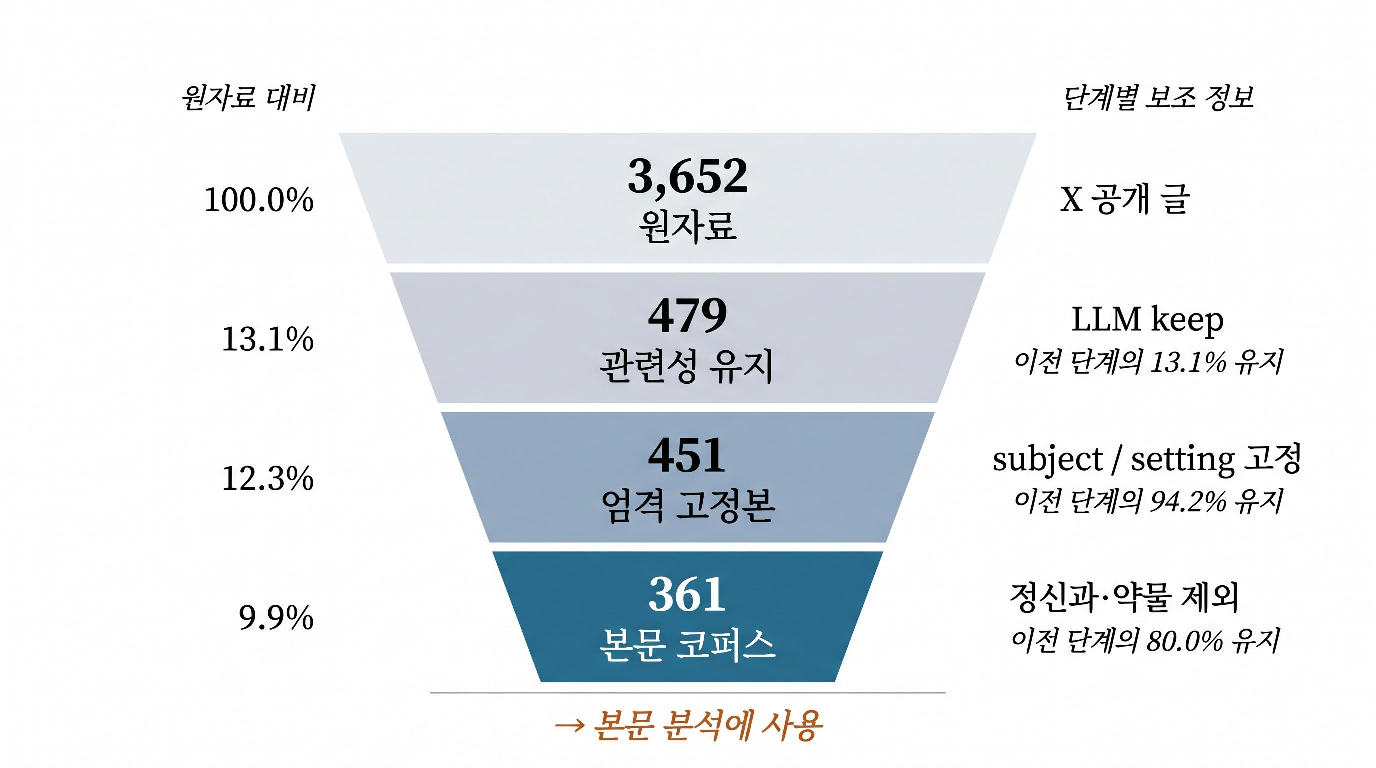
\includegraphics[width=0.76\columnwidth]{figures/corpus_funnel.pdf}
    \captionsetup{width=\columnwidth}
    \caption{원자료 3{,}652건이 본문 코퍼스 361건으로 좁혀지는 정제 단계. 관련성 유지본 479건, 엄격 확정본 451건을 거쳐 본문 코퍼스 361건(원자료의 9.9\%)이 분석에 사용되었다.}
    \label{fig:funnel}
\end{figure}


    \heading{분석 틀}
    분석 틀은 두 층이다. \textbf{이론 고정층}은 작업동맹의 세 축(유대$\cdot$과제$\cdot$목표)이고, \textbf{탐색 고정층}은 여섯 과정 코드(강제성$\cdot$무시당함$\cdot$상처$\cdot$이해받음$\cdot$안도$\cdot$성장)의 이진 등장 여부다. 결과의 안정성은 \textbf{부트스트랩 재표집}과 \textbf{LLM 비의존 점검}으로 확인했다.
  \end{block}

\end{column}

\separatorcolumn

% ============================================================
% RIGHT COLUMN
% ============================================================
\begin{column}{\colwidth}

% ---------------- Results ----------------
  \begin{block}{연구 결과}

    \heading{기초 분포}
    본문 코퍼스 361건의 경험 극성은 부정 117$\cdot$혼합 91$\cdot$긍정 126$\cdot$중립 27건으로, 부정과 긍정이 거의 같은 비중으로 함께 들어왔다. 장면은 일반 정신건강 상담 268건과 청소년 학교상담 93건(약 26\%)으로 나뉘었다.
    \begin{figure}[h]
    \centering
    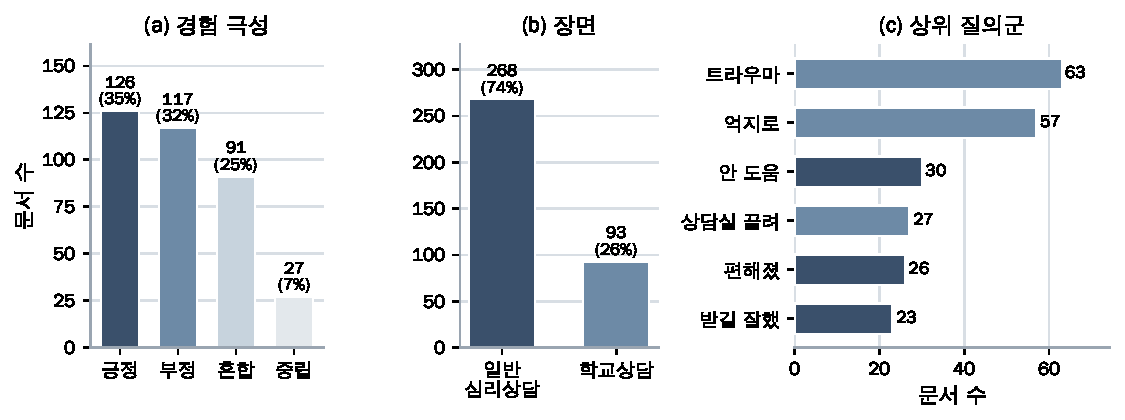
\includegraphics[width=\columnwidth]{figures/corpus_overview.pdf}
    \captionsetup{width=\columnwidth}
    \caption{본문 코퍼스 361건의 분포. (a) 경험 극성: 긍정 126$\cdot$부정 117$\cdot$혼합 91$\cdot$중립 27건으로 부정과 긍정이 비슷한 비중을 차지한다. (b) 장면: 일반 정신건강 상담 268건, 청소년 학교상담 93건(약 26\%). (c) 상위 질의군에는 파열 경험(트라우마$\cdot$억지로$\cdot$안 도움)과 회복 경험(편해졌$\cdot$받길 잘했)이 함께 나타난다.}
    \label{fig:overview}
\end{figure}


    \heading{면접 기반 선행 연구와의 비교}
    \begin{table}[h]
  \centering
  \caption{면접 기반 선행 연구와 본 SNS 자료의 분포 비교. 본 연구의 과정 코드는 문보경$\cdot$장성숙(2001)의 범주를 출발점으로 만든 것이며, 두 자료원의 결과가 같은 모집단의 일치를 의미하지는 않는다.}
  \label{tab:compare}
  \small
  \begin{tabularx}{\columnwidth}{@{}>{\raggedright\arraybackslash}p{0.16\columnwidth} >{\raggedright\arraybackslash}X >{\raggedright\arraybackslash}X@{}}
    \toprule
    \textbf{측면} & \textbf{면접 자료 (문보경$\cdot$장성숙, 2001)} & \textbf{본 SNS 자료} \\
    \midrule
    자료원 & 내담자 면접$\cdot$개방형 질문지 & 한국어 공개 X 경험 글 \\
    분석 단위 & 사례 단위 사건 회고 & 게시물 단위 경험 글 \\
    부정 표지 & 원치 않는 반응, 해결책 부재, 상담자의 요구, 상처 경험 & 강제성 0.350, 무시당함 0.470, 상처 0.231 (부정 117건 기준) \\
    분석 깊이 & 사례별 깊이 있는 합의 부호화 & 분포 수준의 탐색적 부호화 \\
    \bottomrule
  \end{tabularx}
\end{table}


    \heading{과정 코드의 극성별 대비}
    부정 경험 117건에서는 작업동맹 유대 63.2\%$\cdot$과제 69.2\%$\cdot$목표 59.0\%가 부정 정렬, 긍정 경험 126건에서는 유대 80.2\%$\cdot$과제 81.7\%$\cdot$목표 84.9\%가 긍정 정렬이었다. 여섯 과정 코드의 대비는 부트스트랩에서 모두 0을 가로지르지 않았다(예: 무시당함 $-0.431$ [$-0.506$, $-0.350$], 안도 $+0.434$ [$0.344$, $0.517$]).
    \begin{figure}[h]
    \centering
    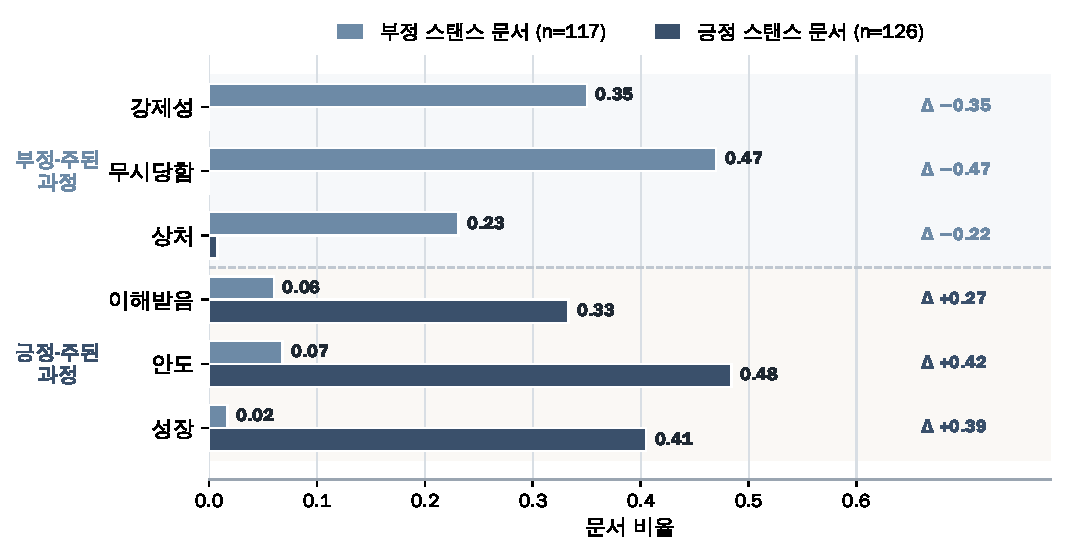
\includegraphics[width=\columnwidth]{figures/process_contrast.pdf}
    \captionsetup{width=\columnwidth}
    \caption{부정 경험(n=117)과 긍정 경험(n=126)의 과정 코드 대비. 부정 경험에서는 무시당함(0.47)$\cdot$강제성(0.35)$\cdot$상처(0.23)가, 긍정 경험에서는 안도(0.48)$\cdot$성장(0.41)$\cdot$이해받음(0.33)이 두드러진다. 여섯 코드의 부트스트랩 신뢰구간은 모두 0을 가로지르지 않았다.}
    \label{fig:process}
\end{figure}


  \end{block}

% ---------------- Conclusions ----------------
  \begin{exampleblock}{결론}
    \begin{itemize}
      \item \textbf{정제 절차의 제안:} 규칙 기반 선별과 LLM 판정을 결합한 4층 정제 절차로 한국어 공개 SNS 상담 경험 자료를 처음으로 본문 코퍼스(361건)로 정리했다.
      \item \textbf{부정$\cdot$긍정 공존:} 정식 표본에서 과소표집되던 부정 경험이 익명 환경에서는 긍정 경험과 거의 같은 비중으로 함께 기록되었다.
      \item \textbf{사건 언어의 구분:} 부정 경험은 ``끌려감$\cdot$무시당함$\cdot$상처받음'', 긍정 경험은 ``이해받음$\cdot$안도$\cdot$변화''의 구조로 분포 수준에서 구분되며, 면접 기반 선행 연구(문보경$\cdot$장성숙, 2001)와 유사한 형태로 나타났다.
      \item \textbf{한계와 전망:} 본 결과는 사람 합의 코딩 부재와 표집 편향의 한계 위에서 관찰된 기술적 사례 보고이며, 후속 합의적 질적 연구와 면접$\cdot$SNS 직접 비교 연구의 출발 자료로 쓸 수 있다.
    \end{itemize}
  \end{exampleblock}

\end{column}
\separatorcolumn

\end{columns}
\end{frame}

\end{document}
